%% Do not edit unless you really know what you are doing.
\documentclass[twoside,english]{report}
\usepackage[sc]{mathpazo}
\usepackage[scaled=0.9]{helvet}
\renewcommand{\ttdefault}{lmtt}
\usepackage[T1]{fontenc}
\usepackage[latin9]{inputenc}
\usepackage[a4paper]{geometry}
\geometry{verbose,lmargin=2cm,rmargin=2cm}
\usepackage{fancyhdr}
\pagestyle{fancy}
\setcounter{secnumdepth}{3}
\setcounter{tocdepth}{3}
\setlength{\parskip}{\smallskipamount}
\setlength{\parindent}{0pt}
\usepackage{babel}
\usepackage{nomencl}

% the following is useful when we have the old nomencl.sty package
\providecommand{\printnomenclature}{\printglossary}
\providecommand{\makenomenclature}{\makeglossary}
\makenomenclature
\usepackage[unicode=true,
 bookmarks=true,bookmarksnumbered=false,bookmarksopen=false,
 breaklinks=false,pdfborder={0 0 1},backref=false,colorlinks=false]
 {hyperref}
\usepackage{breakurl}

%%COMMENTARE PRIMA DI PUBBLICARE 
%----------------------------------------------------------------
\usepackage{draftwatermark} %per il watermark sullo sfondo
%----------------------------------------------------------------
% Per mettere dei commenti per revisione si possono usare i comandi:
% \unsure per le parti in cui non si � sicuri
% \change per le parti che devono essere cambiate in fase di revisone
% \improvement per le parti che devono essere descritte meglio
% \info per scrivere un commento informativo
% \thiswillnotshow � un commento che viene visto solo nel punto in cui viene piazzato e non nella lista delle note
%----------------------------------------------------------------

\makeatletter


% Customization file for the titlepage and document
%************************************************************
% Required stuff
%************************************************************
\usepackage{graphicx}
\usepackage{euler}
\usepackage[detect-all]{siunitx}
\usepackage{sectsty}
\usepackage[font={footnotesize }]{caption}
\usepackage{multicol}
\usepackage{prettyref}

\allsectionsfont{\rmfamily}

% Page customization
\usepackage{fancyhdr}
\pagestyle{fancy}

% Color
\usepackage{color}
\definecolor{light-gray}{gray}{0.85}
\definecolor{dark-gray}{gray}{0.75}

\fancyhead{}  % clear all header fields
\fancyhead[LO,RE]{\rule[-2ex]{0pt}{2ex}\fontsize{9}{11} \selectfont \myPhase}
\fancyhead[RO,LE]{\raisebox{-0.35cm}{
\includegraphics[height=1.2cm,keepaspectratio]{gfx/Logo_TotalBlack.pdf}}}
\fancyhead[CO,CE]{\fontsize{9}{11} \selectfont \myIPT}
\fancyfoot{}  % clear all footer fields
\fancyfoot[RO,LE]{\fontsize{5.5}{8} \selectfont This work is to be considered classified. The use is allowed only for Skyward Experimental Rocketry related activities and projects. For public access please contact \href{mailto:info@skywarder.eu}{info@skywarder.eu}}
\fancyfoot[RE,LO]{\fontsize{9}{11} \selectfont \thepage}
\fancyheadoffset[LE,RO]{0.2pt}
\renewcommand{\headrulewidth}{0.2pt}
\renewcommand{\footrulewidth}{0.2pt}
\renewcommand{\headrule}{\hbox to\headwidth{%
   \leaders\hrule height \headrulewidth\hfill}}
\renewcommand{\footrule}{\hbox to\headwidth{%
    \leaders\hrule height \headrulewidth\hfill}}
\hypersetup{colorlinks=true, linkcolor=blue ,linktoc=page,citecolor=black}

\usepackage{pdfpages} %per includere pdf di più pagine


% Custom notes
\usepackage{xargs}                      % Use more than one optional parameter in a new commands
\usepackage[pdftex,dvipsnames]{xcolor}  % Coloured text etc.

\usepackage[colorinlistoftodos,prependcaption,textsize=tiny]{todonotes}
\newcommandx{\unsure}[2][1=]{\todo[linecolor=red,backgroundcolor=red!25,bordercolor=red,#1]{#2}}
\newcommandx{\change}[2][1=]{\todo[linecolor=blue,backgroundcolor=blue!25,bordercolor=blue,#1]{#2}}
\newcommandx{\info}[2][1=]{\todo[linecolor=OliveGreen,backgroundcolor=OliveGreen!25,bordercolor=OliveGreen,#1]{#2}}
\newcommandx{\improvement}[2][1=]{\todo[linecolor=Plum,backgroundcolor=Plum!25,bordercolor=Plum,#1]{#2}}
\newcommandx{\thiswillnotshow}[2][1=]{\todo[disable,#1]{#2}}
\reversemarginpar
\setlength{\marginparwidth}{2cm}
%End custom notes


%************************************************************
% Redefining numbering for sections
%************************************************************
%\renewcommand*\thesection{\arabic{section}}

%************************************************************
% Cross reference set-up
%************************************************************
\newrefformat{tab}{Table\,\ref{#1}}
\newrefformat{fig}{Figure\,\ref{#1}}
\newrefformat{eq}{Eq.\,\textup{(\ref{#1})}}
\newrefformat{sec}{Sec.\,\ref{#1}}
\newrefformat{sub}{Sec.\,\ref{#1}}

%************************************************************
% Fancy stuff
%************************************************************
\newcommand{\titlecap}[1]{\Huge{\textrm{#1}}}
\newcommand{\subtitlecap}[1]{\Large{\textsc{#1}}}
\newcommand{\sscap}[1]{\textbf{#1}}
\newcommand{\strong}[1]{\textbf{#1}}
\setlength{\headheight}{60pt} %%or

%************************************************************
% Helpful stuff to modify here, not in the LyX Document
%************************************************************
\newcommand{\myDate}{\today}
\newcommand{\myGroup}{Skyward Experimental Rocketry}
\newcommand{\myUrl}{\url{http://www.skywarder.eu}}
\newcommand{\myUni}{Politecnico di Milano}

\newcommand{\myPhase}{Riassunto globale}
\newcommand{\myProject}{Advanced Operating Systems}
\newcommand{\myIPT}{Electronic Systems\\ Integrated Project Team}
\newcommand{\myTitle}{Riassunto}
\newcommand{\myAuthor}{Matteso}
\newcommand{\myEditor}{Nobody}
\newcommand{\myEmail}{XX@skywarder.eu}

\newcommand{\mail}[1]{\href{mailto:#1}{\texttt{#1}}}

\makeatother

\begin{document}
\thispagestyle{empty}
\pdfbookmark{Titlepage}{Titlepage}

\vspace{3cm}
\begin{center}
\bigskip
\Large{\myDate}
\vspace{0.5cm}

{\titlecap{Project \myProject} \\
\vspace{0.3cm}
\titlecap{\myPhase}}\\
\vspace{0.4cm}
\rule{\linewidth}{0.5mm}
\titlecap{\myTitle}
\end{center}

\vfill
\begin{multicols}{2}
\centering{

\includegraphics[height=4cm]{gfx/Logo_Colour.pdf} \\

\includegraphics[height=3cm]{gfx/Logo_Polimi}
}
\vfill
\columnbreak
{\centering{
	\subtitlecap{\myIPT} \\
	\vspace{0.7em}
	\normalsize
	\textrm{\myGroup \\
	\myUni }}}
\vfill

\raggedright{\textbf{Author}: {\myAuthor}\\
\textbf{Editor}: {\myEditor}}

						
\end{multicols}

\clearpage

%*******************************************************
% Titleback
%*******************************************************
\thispagestyle{empty}

\hfill
\vspace{5cm}

\strong{Abstract}\\
Scrivi qui il tuo abstract
\vfill

\begin{multicols}{2}
\medskip
\noindent{\sscap{Website}}: \\
\url{http://www.skywarder.eu}


\medskip
\noindent{\sscap{E-mail}}: \\
\mail{\myEmail}
\vfill
\columnbreak
\section*{Restricted use policy}
\fontsize{8}{11} \selectfont This report is developed during the activities done within Skyward Experimental Rocketry association. Its use is allowed only for Skyward Experimental Rocketry related purposes. If you're a Skyward member, please don't send or release publicly this file without previous acceptance from Direction Board.
For public access and publication please contact \href{mailto:info@skywarder.eu}{info@skywarder.eu}.
\end{multicols}
\vspace{1cm}
\hrule
\bigskip
\clearpage


\pagenumbering{roman}

\begin{multicols}{2}

\printnomenclature{}

\end{multicols}

\tableofcontents{}

\listoffigures


\listoftables

%%COMMENTARE PRIMA DI PUBBLICARE 
%----------------------------------------------------------------
\listoftodos[Notes] %per avere l'elenco delle note
%----------------------------------------------------------------

\clearpage{}

\pagenumbering{arabic}

\setcounter{page}{1}

\global\long\def\diff{\text{d}}



\chapter{GitHub}
\section{initialize repository}
\begin{itemize}
\item \textbf{git init}, create a new folder with files 
\item \textbf{git add $<files>$}, with "." add every file in the folder, "*.tex" just the \LaTeX   files.
\item \textbf{git commit .}, commits every file in the folder.
\item \textbf{git remote add $<repo name>$ $<repo url>$},create a new repo on github website
\item \textbf{git push -u $<repo name>$  $<branch name>$}
\end {itemize}


\section{work on repository}
\begin{itemize}
\item \textbf{git add} $<file to add to staging area>$
\item \textbf{git commit -m "comment" }, commits locally the changes, adding an inline comment.
\item \textbf{git push -u$<repo name>$ $<branch name>$}, the "-u" is needed only if you want to commit from a specific user.
\end{itemize}

\section{remote repository management}
\begin{itemize}
\item \textbf{git clone $<repository\ url>$} downloads the full remote repository to the local computer, but has to be done on an empty folder.
\item \textbf{git fetch $<repository\ name>$}, downloads the full remote repository to the local computer, overwriting the local files.
\item \textbf{git pull $<repository\ name>$ $[branch\ name]$}, downloads the changes from the remote repository.
\item \textbf{git push -u $<repository\ name>$ $[branch\ name]$}, uploads the changes to the remote repository.
\end{itemize}

\section{General use}
\begin{itemize}
	\item \textbf{git status}, gives information about the changes in the local folder.
	\item \textbf{git log}, gives information about all the commits of the repository, with each comment.
\end{itemize}

\section{Branch}
\subsection{Create a new Branch}
\begin{itemize}
\item \textbf{git checkout -b $<new\ branch\ name>$}
\item \textbf{git stauts}
\item \textbf{git add $<file\ to\ commit>$}
\item \textbf{git commit -m "comment"}
\item \textbf{git push -u $<repo\ name>$ $<new\ branch\ name>$}
\end{itemize}
\subsection{Merge Branch with master}
\begin{itemize}
	\item \textbf{git checkout master}, move to the master branch (or whatever branch you want to merge with).
	\item \textbf{git merge $<branch\ name>$}, merges the specified branch with the actual branch.
\end{itemize}


\subsection{switch to an other branch}
\begin{itemize}
\item \textbf{git checkout $<branch\ name>$}
\end{itemize}

\section{Undo Commands}
\begin{itemize}
\item \textbf{git reset - -hard}, delete changes to the last commit
\item \textbf{git commit --amend}, change a commit
\item \textbf{revert $<SHA-1 number>$}, revert to a specific commit
\end{itemize}



\begin{figure}[h]
	\centering
	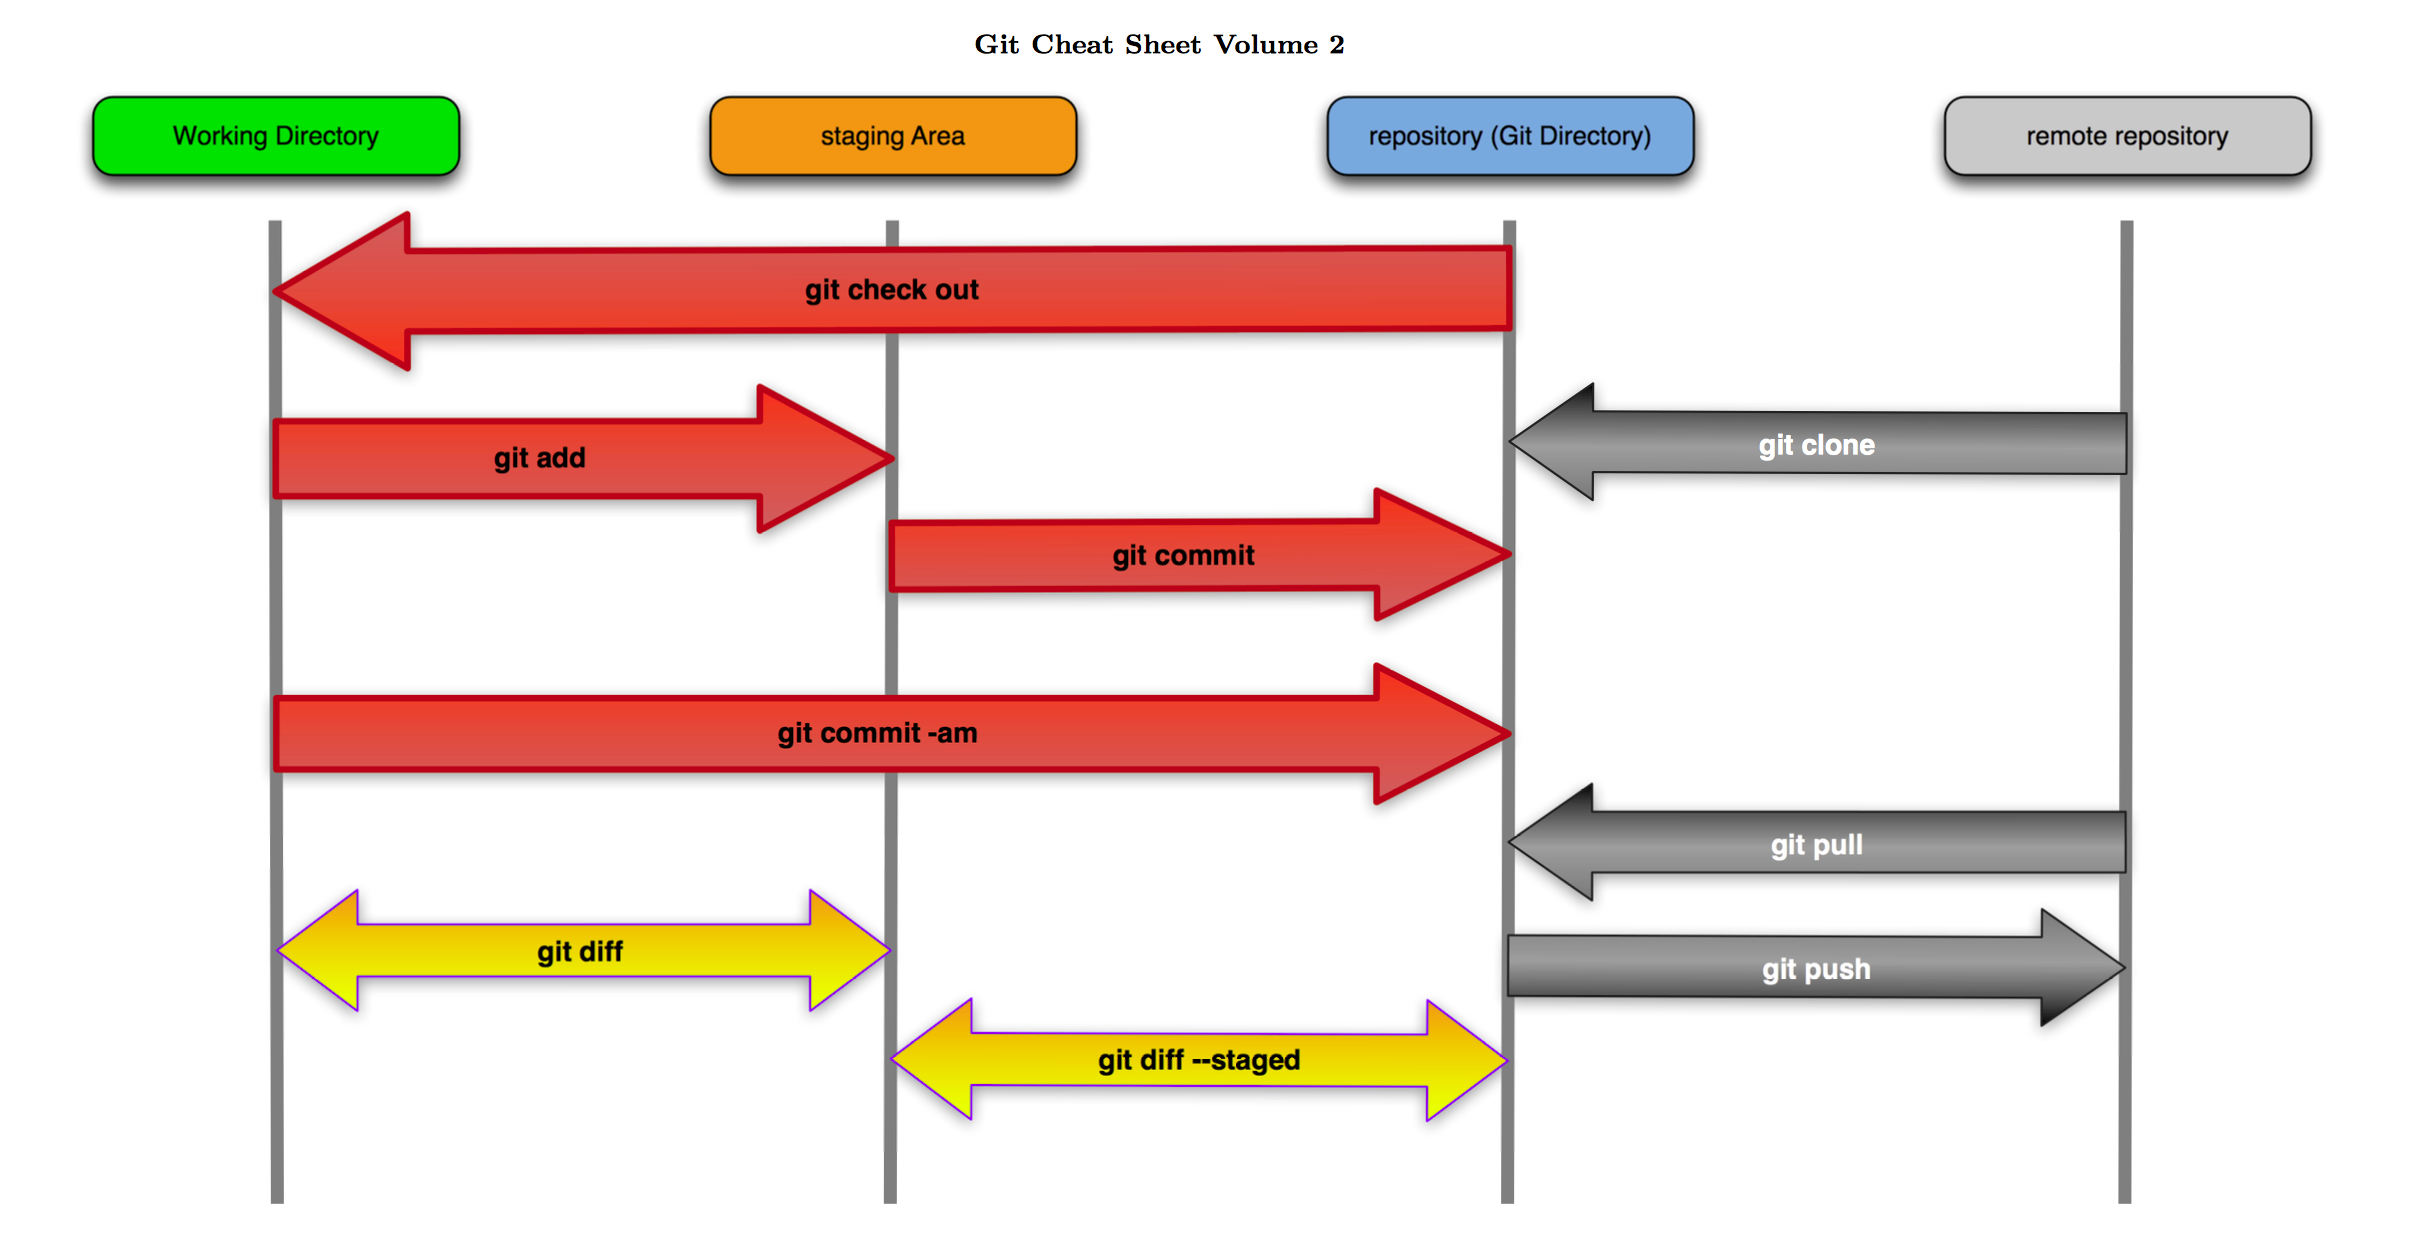
\includegraphics[width=\textwidth]{gfx/git_graph}
	
	\caption{Comandi GIT}
	\label{Fig:Commands}
\end{figure}


\chapter{Scheduling}
\section{Criteria}
\begin{itemize}
\item \textbf{CPU utilization}, keep CPU as busy as possible
\item \textbf{throughput}, number of processes that complete their execution per time unit
\item \textbf{turnaround time}, amount of time to execute a particular process
\item \textbf{waiting time}, amount of time a process has been waiting in the ready queue
\item \textbf{response time}, amount of time it takes from when a request was submitted until the first response is produce, not output

\end{itemize}
\section{Algorithms}
A detailed description is provided in Table \ref{Tab:Algorithms}.
\begin{table}[]
	\centering
	\resizebox{\textwidth/4*3}{!}{%
		\begin{tabular}{|p{\textwidth/11}|p{\textwidth/10}|p{\textwidth/11}|p{\textwidth/11}|p{\textwidth/11}|p{\textwidth/11}|p{\textwidth/11}|p{\textwidth/11}|p{\textwidth/9}|p{\textwidth/9}|p{\textwidth/8}|}
			\hline
			\textbf{Scheduler}                   & \textbf{Preemptive} & \textbf{Priority} & \textbf{CPU Utilization} & \textbf{Thrughput} & \textbf{Turnaround time}                             & \textbf{Waiting time}                           & \textbf{Response time}                          & \textbf{Advantages}                                                                                                                    & \textbf{Issues}                                                                                         & \textbf{Description}                                                                                                       \\ \hline
			First Come First Served (FCFS)       & NO                  & NO                & LOW                      & LOW                & SHORTEST                                             & HIGH                                            & HIGH                                            & Semplicity                                                                                                                             & Processes may starve if after long process                                                              & Favours CPU-bound processes                                                                                                \\ \hline
			Shortest Job First (SJF)             & NO                  & NO                & HIGH                     & HIGH               & LONG for long processes, SHORTEST for fast processes & HIGH for long processes, LOW for fast processes & HIGH for long processes, LOW for fast processes & Minimum Average Waiting time                                                                                                           & Long processes may starve, must estimate process time: not implementable in most cases for this reason. & Favours the processes that need less CPU-time                                                                              \\ \hline
			Shortest Remaining Time First (SRTF) & YES                 & NO                & HIGH                     & HIGH               & LONG for long processes, SHORTEST for fast processes & MEDIUM                                          & MEDIUM                                          & If a shorter task is available, it runs immediately in CPU, less overhead (the scheduler decides only when another process approaches) & Long processes may starve (worst than SJF), must estimate process time.                                 & It's the SJF but with preemption                                                                                           \\ \hline
			Higher Response Ratio Next           & NO                  & YES               & HIGH                     & MEDIUM             & MEDIUM                                               & LOW                                             & MEDIUM                                          & Prevents starvation by assigning higher priority to processes waiting for a long time.                                                 & must estimate process time                                                                              & It's the evolution of SJF.                                                                                                 \\ \hline
			Feedback                             & YES                 & NO                & HIGH                     & LOW                & LONG                                                 & LOW                                             & LOW                                             & No starving processes, don't know remaining time process needs to execute.                                                             & High overhead and continuous context switch                                                             & Penalizes jobs that have been runnning longer                                                                              \\ \hline
			Fair-Share Scheduling (FSS)          & YES                 & NO                & LOW                      & LOW                & LONG                                                 & LOW                                             & LOW                                             & Every process has its fair share of CPU time, useful with multiple group users.                                                        & Processes in crowded groups get less CPU time                                                           & Applies the round-robin scheduling strategy at each level of abstraction (processes, users, groups, etc.)                  \\ \hline
			Round Robin                          & YES                 & NO                & HIGH                     & MEDIUM             & LONG                                                 & LOW                                             & LOW                                             & No starvation, equal waiting time                                                                                                      & Longer turnaround time (every process takes longer if slower than a time quantum)                       & Uses preemption based on a clock, every process is executed in 1 time quantum and than leaves the CPU to the next process. \\ \hline
		\end{tabular}%
	}
	\caption{Main Scheduling Algorithms}
	\label{Tab:Algorithms}
\end{table}

\chapter{TDE Questions}
\section{Describe the general characteristics of a scheduling for real-time, possibly including a comparison between Rate Monotonic and EDF. }



\section{Describe the general characteristics and figures of merit of a CPU scheduler and those more related to the case of Real Time Operating Systems}
\section{Describe the ARM Cortex-M processor by detailing its main features, its registers and the organization and functional principle of the vector table. Extra: What is the CMSIS and which are its main purposes?  }
Q1 See presentation ARM Processors and Architectures - Introduction and Programmer's Model
\section{Describe how interrupts work, detailing the difference between a simple interrupt and one where a context switch occurs.}
Interrupts provide a way to interrupt the normal program flow of the CPU  to handle events generated by peripherals without the expense of polling. A contex switch implies an operating system. In a bare metal embedded device without operating system, no context switch exist. In this case, the interrupt interrupts the execution of the main code (i.e, of the main() function or of a function who is in the call stack of main()). When there is no context switch, the only registers that need to be saved are the ones used by the interrupt service routine (ISR), because at the end of the ISR the code execution will return to the main code, which can be thought of as the only task in the system. This register saving is often done by the compiler. 
This is the timeline:  
++ main code | ISR | main code ++> Time

When you add an OS, an interrupt can wake up a higher priority task than the currently running one (or the time quantum of the task can be expired). So, the task that is running at the end of the interrupt may not be the same as the one running before, as in this timeline: 


++ task1 | ISR | task2 ++> Time


Since each task has its set of registers, upon entering the ISR all registers have to be stored in a per­task data structure within the OS, called a task control block. This is because the registers that will be restored at the end of the ISR will be those of the next task, which may or may not be the one that was interrupted. Not saving all of them (or not restoring all of them) does not work when the before and after task differ. This saving is done by code in the OS, not by the compiler.

\section{title}
\section{title}

%inserire un PDF nel pdf
%\begin{figure}[h]
%	\centering
%	\includegraphics[scale=1]{doc/nome_del_documento}
%	
%	\caption{descrizione, se necessaria}
%	\label{Fig:etichetta_documento}
%\end{figure}

\end{document}
